\documentclass{article}
\usepackage{mathtools}
\usepackage{graphicx} % Required for inserting images
\usepackage[a4paper, total={7in, 9in}]{geometry}
\usepackage{minted}
\usepackage{amsfonts} % Add this line to include the amsfonts package
\usepackage{datetime} % For date if required


\usepackage{algorithm}
\usepackage{algpseudocode} % Part of algorithmicx package

\usepackage{amsmath}
\DeclareMathOperator*{\argmin}{arg\,min}  % The asterisk is used to place the subscript under "arg min" in display style


\setlength\parindent{0pt}


\title{BIOMATH 208 Comp Exam Attempts}
\author{Simon A. Lee}
\date{}

\begin{document}

\maketitle

\section{Chapter 1}
\subsection{Discreet images and interpolation}
\textbf{Calculating Sample Values}

Given the formula \( I_i = 1 - (i - 2)^2 \), let's calculate the values for each sample:

\begin{itemize}
    \item For \( i = 0 \): \( I_0 = 1 - (0 - 2)^2 = 1 - 4 = -3 \)
    \item For \( i = 1 \): \( I_1 = 1 - (1 - 2)^2 = 1 - 1 = 0 \)
    \item For \( i = 2 \): \( I_2 = 1 - (2 - 2)^2 = 1 - 0 = 1 \)
    \item For \( i = 3 \): \( I_3 = 1 - (3 - 2)^2 = 1 - 1 = 0 \)
    \item For \( i = 4 \): \( I_4 = 1 - (4 - 2)^2 = 1 - 4 = -3 \)
\end{itemize}

The pixel locations are \( x_i = O + i\Delta = -0.5 + 0.25i \), specifically:
\begin{itemize}
    \item \( x_0 = -0.5 \)
    \item \( x_1 = -0.25 \)
    \item \( x_2 = 0 \)
    \item \( x_3 = 0.25 \)
    \item \( x_4 = 0.5 \)
\end{itemize}

\textbf{Evaluating Image at \( x = 0.1 \)}

Using linear interpolation between \( x_1 = -0.25 \) and \( x_2 = 0 \), where \( I_1 = 0 \) and \( I_2 = 1 \):

The equation for the line between these two points can be derived from:

\[
y = y_1 + \frac{(y_2 - y_1)}{(x_2 - x_1)} (x - x_1)
\]

Substituting in our values:

\[
y = 0 + \frac{(1 - 0)}{(0 - (-0.25))} (0.1 - (-0.25))
\]

\[
y = 4 \times (0.1 + 0.25) = 4 \times 0.35 = 1.4
\]

Hence, \( I(0.1) = 1.4 \).

\begin{figure}[h!]
    \centering
    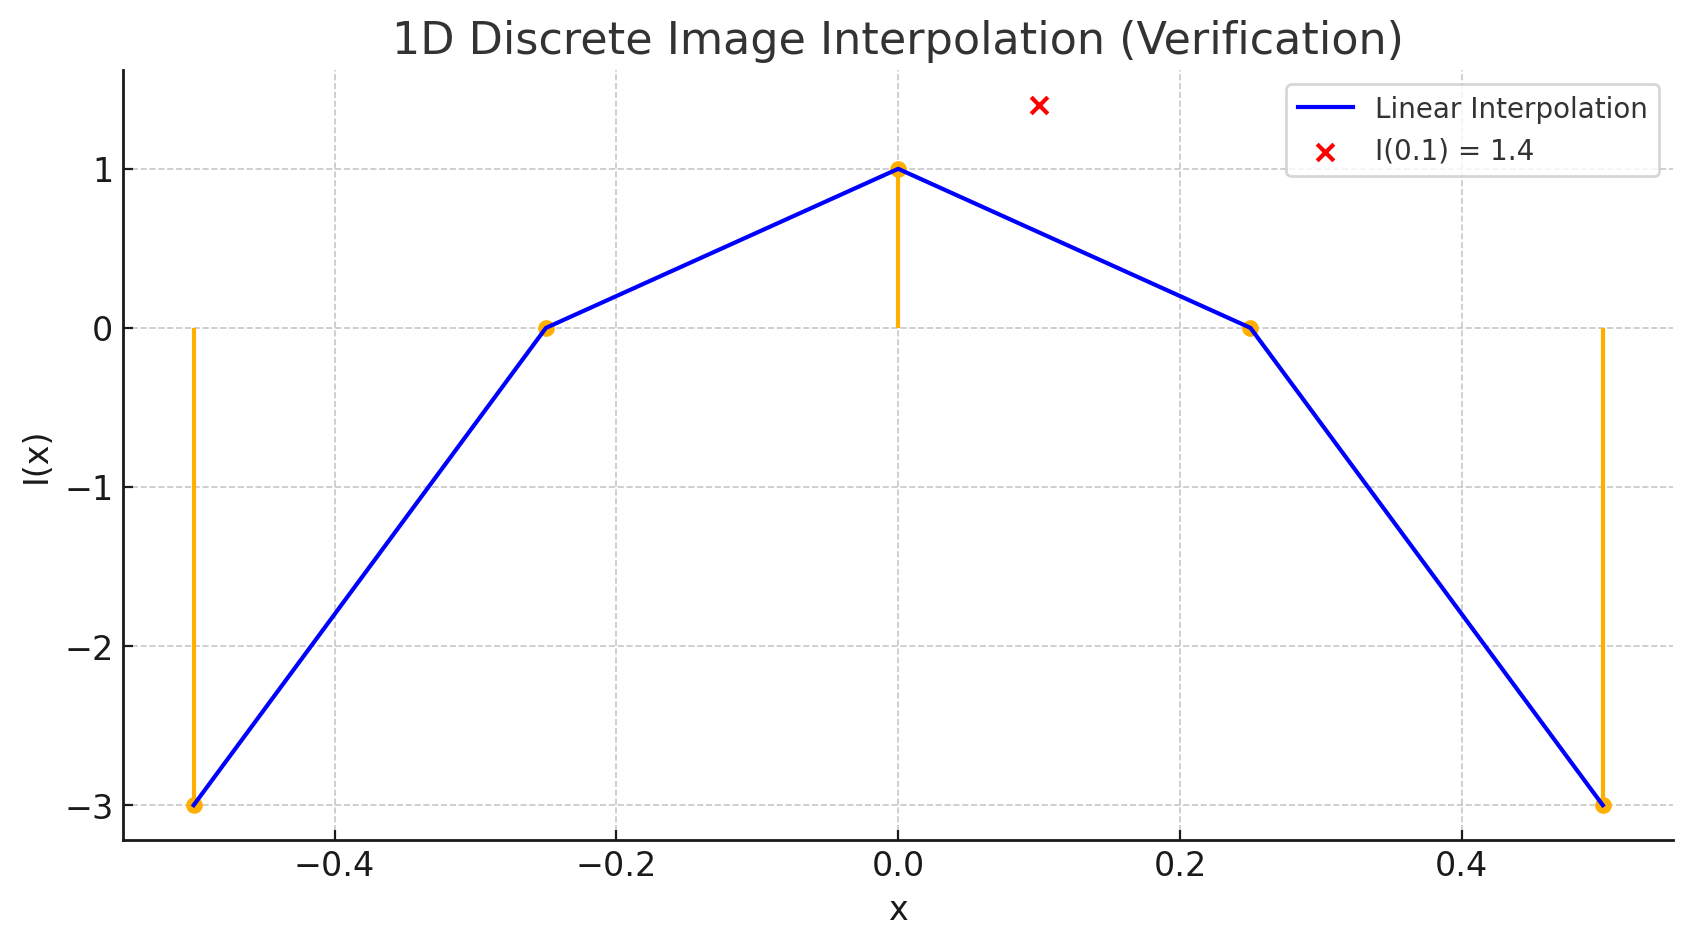
\includegraphics[width=0.5\linewidth]{fig1.png}
    \caption{fig1}
\end{figure}

\subsection{Color maps}

\textbf{Matching the Images:}
\begin{enumerate}
    \item 1. Image 1: Dominant blue in the middle layers (cortex and white matter) and light gray for the outermost layer (skull). This suggests that blue should be prominent in middle brightness values and red should be high for the highest brightness. This matches Colormap D.
    \item 2. Image 2: Prominently red in the innermost areas (ventricles), with other regions in different colors. This suggests the red channel is emphasized in lower brightness, fitting Colormap C.
    \item 3. Image 3: Predominantly green for the middle layers, indicating a colormap where green is emphasized in middle brightness values. This matches Colormap B.
    \item 4. Image 4: This image is shaded with a consistent color pattern from dark to light gray, suiting a colormap where the red channel is high across most values, matching Colormap A.
\end{enumerate}

### Conclusion:
\begin{itemize}
    \item - A corresponds to 4
    \item - B corresponds to 3
    \item - C corresponds to 2
    \item - D corresponds to 1
\end{itemize}

\newpage
\section{Chapter 2}
\subsection{Change of covector components}

\textbf{Step 1: Express the Covector in Standard Coordinates}
Given the basis \(A\) where \(A_0 = (1,0)\) and \(A_1 = (1,-1)\), the covector \(\mu\) in the standard coordinate system is expressed as:
\[
\mu = \mu_0 A^0 + \mu_1 A^1
\]
Given \(\mu_0 = 1\) and \(\mu_1 = 1\), the basis vectors \(A^0\) and \(A^1\) are the duals of \(A_0\) and \(A_1\). The dual basis vectors can be found by ensuring they satisfy \(A^i \cdot A_j = \delta^i_j\), where \(\delta^i_j\) is the Kronecker delta.

Since \(A^0\) and \(A^1\) are covectors, and the dual basis vectors correspond to the rows of the inverse of the matrix formed by placing the basis vectors as columns, we can solve for them:
- \(A_0\) and \(A_1\) form the matrix \(\begin{bmatrix} 1 & 1 \\ 0 & -1 \end{bmatrix}\).
- The inverse of this matrix, whose rows will be the dual basis vectors, is:
  \[
  \begin{bmatrix} 1 & 1 \\ 0 & -1 \end{bmatrix}^{-1} = \begin{bmatrix} 1 & 1 \\ 0 & -1 \end{bmatrix}
  \]
  Therefore, \(A^0 = (1, 0)\) and \(A^1 = (1, -1)\).

Hence, the covector \(\mu\) in standard coordinates is:
\[
\mu = 1 \cdot (1, 0) + 1 \cdot (1, -1) = (1+1, 0-1) = (2, -1)
\]

\textbf{Step 2: Express the Covector in the Basis \(B\)}
Basis \(B\) consists of \(B_0 = (0, -1)\) and \(B_1 = (-1, 1)\). We now need to express the vector \((2, -1)\) in terms of \(B_0\) and \(B_1\). This requires solving the equation:
\[
(2, -1) = \mu^B_0 (0, -1) + \mu^B_1 (-1, 1)
\]
Let's set up the equations:
1. \(0 \cdot \mu^B_0 - \mu^B_1 = 2\)
2. \(-\mu^B_0 + \mu^B_1 = -1\)

Solving this system of linear equations:
- Adding both equations, we get:
  \[
  0 = 1 \implies \mu^B_1 - \mu^B_0 = 1
  \]
- From the first equation:
  \[
  -\mu^B_1 = 2 \implies \mu^B_1 = -2
  \]
- Substitute \(\mu^B_1\) in the equation derived from the sum:
  \[
  -\mu^B_0 - 2 = 1 \implies \mu^B_0 = -3
  \]

\newpage
\section{Chapter 3}
\subsection{Inner Product}
First, let's calculate the centers and area-weighted normals for each surface:
\textbf{Surface 1}
Center:
$$[c_1 = \left(\frac{1}{3}, \frac{1}{3}, 0\right)]$$
Area-weighted normal:
$$[A_1 = \frac{1}{2}(1,0,0) \times (0,1,0) = \left(0, 0, \frac{1}{2}\right)]$$
\textbf{Surface 2}
Center:
$$[c_2 = \left(0, \frac{1}{3}, \frac{1}{3}\right)]$$
Area-weighted normal:
$$[A_2 = \frac{1}{2}(0,0,1) \times (0,1,0) = \left(\frac{1}{2}, 0, 0\right)]$$
Now, let's compute the inner product:
$$[k(c_1 - c_2) = \exp\left(-\frac{|\left(\frac{1}{3}, 0, -\frac{1}{3}\right)|^2}{2\sigma^2}\right) = \exp\left(-\frac{2/9}{2\sigma^2}\right)]
[A_1 \cdot A_2 = \left(0, 0, \frac{1}{2}\right) \cdot \left(\frac{1}{2}, 0, 0\right) = 0]$$
The inner product is:
$$[\text{Inner Product} = k(c_1 - c_2) A_1 \cdot A_2 = 0]$$
Note: The inner product is zero due to the orthogonality of the surface normals, which simplifies our calculation significantly.


\subsection{Distance Between Surfaces}
To compute the norm squared of the distance between the two surfaces, we use the formula:
$$[\text{Distance}^2 = \langle A, A \rangle + \langle B, B \rangle - 2\langle A, B \rangle]$$
Where $\langle A, A \rangle$ and $\langle B, B \rangle$ are the inner products of each surface with itself, and $\langle A, B \rangle$ is the inner product between the two surfaces (which we found to be 0).
\textbf{$\langle A, A \rangle$ (Surface 1 with itself)}
$$
[k(c_1 - c_1) = k(0) = 1]
[A_1 \cdot A_1 = \left(0, 0, \frac{1}{2}\right) \cdot \left(0, 0, \frac{1}{2}\right) = \frac{1}{4}]
[\langle A, A \rangle = 1 \cdot \frac{1}{4} = \frac{1}{4}]
$$
\textbf{$\langle B, B \rangle$ (Surface 2 with itself)}
$$
[k(c_2 - c_2) = k(0) = 1]
[A_2 \cdot A_2 = \left(\frac{1}{2}, 0, 0\right) \cdot \left(\frac{1}{2}, 0, 0\right) = \frac{1}{4}]
[\langle B, B \rangle = 1 \cdot \frac{1}{4} = \frac{1}{4}]
$$
\textbf{Final Calculation}
$$
[\text{Distance}^2 = \frac{1}{4} + \frac{1}{4} - 2(0) = \frac{1}{2}]$$
Therefore, the norm squared of the distance between the two surfaces is $\frac{1}{2}$.

\newpage
\section{Chapter 4}
To show that the two charts $x$ and $y$ form a smoothly compatible atlas for the 2D plane, we need to prove that the transition map between them is smooth and invertible.

\subsection{Transition Maps}

Let's define the transition maps:

\begin{align*}
\phi_{yx} &: x \to y \\
\phi_{xy} &: y \to x
\end{align*}

\textbf{Calculating $\phi_{yx}$}

For a point $(p^1, p^2)$ in the body:

\begin{align*}
x(p) &= (p^1, p^2) = (x^0, x^1) \\
y(p) &= (\arctan(p^1/d), p^2) = (y^0, y^1)
\end{align*}

Therefore:

\begin{align*}
\phi_{yx}(x^0, x^1) &= (\arctan(x^0/d), x^1) \\
&= (y^0, y^1)
\end{align*}

\textbf{Calculating $\phi_{xy}$}

Similarly:

\begin{align*}
\phi_{xy}(y^0, y^1) &= (d \tan(y^0), y^1) \\
&= (x^0, x^1)
\end{align*}

\textbf{Smoothness of $\phi_{yx}$}

The Jacobian of $\phi_{yx}$ is:

\[
J_{\phi_{yx}} = \begin{bmatrix}
\frac{\partial y^0}{\partial x^0} & \frac{\partial y^0}{\partial x^1} \\
\frac{\partial y^1}{\partial x^0} & \frac{\partial y^1}{\partial x^1}
\end{bmatrix}
= \begin{bmatrix}
\frac{1}{d(1 + (x^0/d)^2)} & 0 \\
0 & 1
\end{bmatrix}
\]

This Jacobian exists and is continuous for all $(x^0, x^1)$, except when $x^0 \to \infty$. However, in the context of CT imaging, $x^0$ is always finite, so $\phi_{yx}$ is smooth in the relevant domain.

\textbf{Smoothness of $\phi_{xy}$}

The Jacobian of $\phi_{xy}$ is:

\[
J_{\phi_{xy}} = \begin{bmatrix}
\frac{\partial x^0}{\partial y^0} & \frac{\partial x^0}{\partial y^1} \\
\frac{\partial x^1}{\partial y^0} & \frac{\partial x^1}{\partial y^1}
\end{bmatrix}
= \begin{bmatrix}
d \sec^2(y^0) & 0 \\
0 & 1
\end{bmatrix}
\]

This Jacobian exists and is continuous for all $(y^0, y^1)$, except when $y^0 = \pm \frac{\pi}{2}$. However, these values correspond to points at infinity in the $x$ chart, which are not relevant in the imaging context.

\textbf{Invertibility}

The transition maps are clearly invertible, as:

\begin{align*}
\phi_{xy}(\phi_{yx}(x^0, x^1)) &= (x^0, x^1) \\
\phi_{yx}(\phi_{xy}(y^0, y^1)) &= (y^0, y^1)
\end{align*}

\textbf{Conclusion}

The charts $x$ and $y$ form a smoothly compatible atlas for the 2D plane in the context of CT imaging, as their transition maps are smooth and invertible within the relevant domain.

\newpage
\section{Chapter 5}

\begin{enumerate}
\item A scale group (5 points)

To show that the given family of matrices form a group under matrix multiplication, we need to verify the group axioms:

\begin{itemize}
\item Associativity: For any $s, t, u \in \mathbb{R}^+$,
\begin{align*}
(G_s G_t) G_u &= \left(\begin{bmatrix} s^0 & 0 \\ 0 & s^1 \end{bmatrix} \begin{bmatrix} t^0 & 0 \\ 0 & t^1 \end{bmatrix}\right) \begin{bmatrix} u^0 & 0 \\ 0 & u^1 \end{bmatrix} \\
&= \begin{bmatrix} (st)^0 & 0 \\ 0 & (st)^1 \end{bmatrix} \begin{bmatrix} u^0 & 0 \\ 0 & u^1 \end{bmatrix} \\
&= \begin{bmatrix} (stu)^0 & 0 \\ 0 & (stu)^1 \end{bmatrix} \\
&= \begin{bmatrix} s^0 & 0 \\ 0 & s^1 \end{bmatrix} \left(\begin{bmatrix} t^0 & 0 \\ 0 & t^1 \end{bmatrix} \begin{bmatrix} u^0 & 0 \\ 0 & u^1 \end{bmatrix}\right) \\
&= G_s (G_t G_u)
\end{align*}

\item Identity: The identity element is $G_1 = \begin{bmatrix} 1 & 0 \\ 0 & 1 \end{bmatrix}$ since for any $s \in \mathbb{R}^+$,
\begin{align*}
G_s G_1 &= \begin{bmatrix} s^0 & 0 \\ 0 & s^1 \end{bmatrix} \begin{bmatrix} 1 & 0 \\ 0 & 1 \end{bmatrix} = \begin{bmatrix} s^0 & 0 \\ 0 & s^1 \end{bmatrix} = G_s \\
G_1 G_s &= \begin{bmatrix} 1 & 0 \\ 0 & 1 \end{bmatrix} \begin{bmatrix} s^0 & 0 \\ 0 & s^1 \end{bmatrix} = \begin{bmatrix} s^0 & 0 \\ 0 & s^1 \end{bmatrix} = G_s
\end{align*}

\item Inverse: For any $s \in \mathbb{R}^+$, the inverse of $G_s$ is $G_{1/s}$ since
\begin{align*}
G_s G_{1/s} &= \begin{bmatrix} s^0 & 0 \\ 0 & s^1 \end{bmatrix} \begin{bmatrix} (1/s)^0 & 0 \\ 0 & (1/s)^1 \end{bmatrix} = \begin{bmatrix} 1 & 0 \\ 0 & 1 \end{bmatrix} = G_1 \\  
G_{1/s} G_s &= \begin{bmatrix} (1/s)^0 & 0 \\ 0 & (1/s)^1 \end{bmatrix} \begin{bmatrix} s^0 & 0 \\ 0 & s^1 \end{bmatrix} = \begin{bmatrix} 1 & 0 \\ 0 & 1 \end{bmatrix} = G_1
\end{align*}
\end{itemize}

Therefore, the given family of matrices form a group under matrix multiplication.

\item Not a scale group (5 points)

If $s^t \in \mathbb{R}$ instead of $\mathbb{R}^+$, then the inverse axiom is violated. Consider $s = -1$:
\[G_{-1} = \begin{bmatrix} (-1)^0 & 0 \\ 0 & (-1)^1 \end{bmatrix} = \begin{bmatrix} 1 & 0 \\ 0 & -1 \end{bmatrix}\]

But $G_{-1}$ does not have an inverse in the family, since for any $t \in \mathbb{R}$, 
\begin{align*}
G_{-1} G_t &= \begin{bmatrix} 1 & 0 \\ 0 & -1 \end{bmatrix} \begin{bmatrix} t^0 & 0 \\ 0 & t^1 \end{bmatrix} = \begin{bmatrix} 1 & 0 \\ 0 & -t \end{bmatrix} \neq \begin{bmatrix} 1 & 0 \\ 0 & 1 \end{bmatrix} = G_1
\end{align*}

Therefore, with $s^t \in \mathbb{R}$, the given family of matrices do not form a group under matrix multiplication, as the inverse axiom is violated.
\end{enumerate}

\newpage
\section{Chapter 6}

The chart transition map formula is:
\begin{align*}
x' &= \frac{dx}{\sqrt{1+d^2-2dy}} \
y' &= \frac{\sqrt{1+d^2-2dy}-1}{d}
\end{align*}

Given:

The point of interest in the pencil beam chart is (1, -1)
d = 1
Step 1: Plug in the values into the x' formula:
\begin{align*}
x' &= \frac{1 \cdot 1}{\sqrt{1+1^2-2 \cdot 1 \cdot (-1)}} \
&= \frac{1}{\sqrt{1+1+2}} \
&= \frac{1}{\sqrt{4}} \
&= \frac{1}{2}
\end{align*}

Step 2: Plug in the values into the y' formula:
\begin{align*}
y' &= \frac{\sqrt{1+1^2-2 \cdot 1 \cdot (-1)}-1}{1} \
&= \sqrt{1+1+2}-1 \
&= \sqrt{4}-1 \
&= 2-1 \
&= 1
\end{align*}

Therefore, the point (1, -1) in the pencil beam chart maps to the point (1/2, 1) in the fan beam chart.

The angle this vector takes in the fan beam chart y can be calculated using the arctangent:

\begin{align*}
\theta &= \arctan(\frac{y'}{x'}) \
&= \arctan(\frac{1}{1/2}) \
&= \arctan(2) \
&\approx 63.4^\circ
\end{align*}

So the vector takes an angle of approximately 63.4° in the fan beam chart y.

\newpage
\section{Chapter 7}

To solve this problem and find the optimal s1 and s2 that minimize the sum of squared error between SQ and P, I'll set up the variational problem in LaTeX, showing all the math steps.

Given:
\begin{align*}
S &= \begin{pmatrix}
s^1 & 0\\
0 & s^2
\end{pmatrix}\\
SQ &= \begin{pmatrix}
s^1 & 0\\
0 & s^2
\end{pmatrix}
\begin{pmatrix}
q_1^1 & q_1^2\\
q_2^1 & q_2^2
\end{pmatrix} =
\begin{pmatrix}
s^1q_1^1 & s^1q_1^2\\
s^2q_2^1 & s^2q_2^2
\end{pmatrix}
\end{align*}

Objective function:
\begin{align*}
E(s^1,s^2) &= \sum_{i=1}^{2}\sum_{j=1}^{2}(s^iq_i^j - p_i^j)^2\\
&= (s^1q_1^1 - p_1^1)^2 + (s^1q_1^2 - p_1^2)^2 + (s^2q_2^1 - p_2^1)^2 + (s^2q_2^2 - p_2^2)^2
\end{align*}

To minimize the objective function, set partial derivatives to zero:
\begin{align*}
\frac{\partial E}{\partial s^1} &= 2(s^1q_1^1 - p_1^1)q_1^1 + 2(s^1q_1^2 - p_1^2)q_1^2 = 0\\
\frac{\partial E}{\partial s^2} &= 2(s^2q_2^1 - p_2^1)q_2^1 + 2(s^2q_2^2 - p_2^2)q_2^2 = 0
\end{align*}

Solve for s1 and s2:
\begin{align*}
s^1 &= \frac{p_1^1q_1^1 + p_1^2q_1^2}{(q_1^1)^2 + (q_1^2)^2}\\
s^2 &= \frac{p_2^1q_2^1 + p_2^2q_2^2}{(q_2^1)^2 + (q_2^2)^2}
\end{align*}

The optimal solution that minimizes the sum of squared error is:
\begin{align*}
s^1 &= \frac{p_1^1q_1^1 + p_1^2q_1^2}{(q_1^1)^2 + (q_1^2)^2}\\
s^2 &= \frac{p_2^1q_2^1 + p_2^2q_2^2}{(q_2^1)^2 + (q_2^2)^2}
\end{align*}

\newpage
\section{Chapter 8}

8.1 The constant speed geodesic equation (5 points)

\begin{align*}
\ddot{y} &= \frac{2q\dot{q}^2}{1+q^2} = 0 \\
\Rightarrow \dot{q}^2 &= 0 \quad \text{or} \quad 1+q^2 = 0
\end{align*}

Since $1+q^2 > 0$ for all real $q$, we must have $\dot{q}^2 = 0 \Rightarrow \dot{q} = 0$. This means $q$ is constant.

Hint: In 1D the three derivative terms in the geodesic equation are equal (up to a sign), and the inverse of the metric is just its reciprocal.

8.2 Solutions to the geodesic equation (5 points)

Plugging in $q(t) = \tan(at+b)$:

\begin{align*}
\dot{q} &= a \sec^2(at+b) \\
\ddot{q} &= 2a^2 \sec^2(at+b) \tan(at+b)
\end{align*}

Plugging into the geodesic equation:

\begin{align*}
\ddot{y} &= \frac{2q\dot{q}^2}{1+q^2} \\
2a^2 \sec^2(at+b) \tan(at+b) &= \frac{2\tan(at+b)a^2\sec^4(at+b)}{1+\tan^2(at+b)} \\
&= 2a^2 \sec^2(at+b) \tan(at+b)
\end{align*}

The equation is satisfied, so $q(t) = \tan(at+b)$ are solutions for any $a,b \in \mathbb{R}$.

8.3 Pullback metric (5 points)

The tangent vectors are:

\begin{align*}
v_{\theta}^{x} &= -\sin(\theta) \\
v_{\theta}^{y} &= \cos(\theta) 
\end{align*}

Their inner product using the metric $g^{(y)}$:

\begin{align*}
g^{(y)}(v_{\theta},v_{\theta}) &= \sin^2(\theta) g^{(y)}(\partial_x,\partial_x) + \cos^2(\theta) g^{(y)}(\partial_y,\partial_y) \\
&= \sin^2(\theta) + \cos^2(\theta) \\
&= 1
\end{align*}

The inner product using $g^{(x)}$:

\begin{align*}
g^{(x)}(v_{\theta},v_{\theta}) &= v_{\theta}^{x}v_{\theta}^{x}g^{(x)}(\partial_x,\partial_x) + v_{\theta}^{y}v_{\theta}^{y}g^{(x)}(\partial_y,\partial_y) \\
&= (-\sin\theta)(-\sin\theta)(1) + (\cos\theta)(\cos\theta)(1) \\
&= \sin^2(\theta) + \cos^2(\theta) \\
&= 1
\end{align*}

Therefore, the pullback of the metric from $y$ to $x$ using the tangent vectors gives the same inner product as the metric in $x$, demonstrating the invariance of the constant speed geodesics in the two charts.

\newpage
\section{Chapter 9}
To answer this, I will go through the Procrustes algorithm steps as outlined in the problem.

First, compute the Riemannian logarithm of the two data points $\frac{1}{4}$ and $\frac{3}{4}$ with base point $\frac{1}{4}$:

\begin{align*}
\log_{\frac{1}{4}}(\frac{1}{4}) &= \log\left(\frac{\frac{1}{4}}{\frac{1}{4}}\right) - \log\left(\frac{1}{1-\frac{1}{4}}\right) = \log(1) - \log\left(\frac{4}{3}\right) = 0 - \log\left(\frac{4}{3}\right) = -\log\left(\frac{4}{3}\right) \\
\log_{\frac{1}{4}}(\frac{3}{4}) &= \log\left(\frac{\frac{3}{4}}{\frac{1}{4}}\right) - \log\left(\frac{1}{1-\frac{1}{4}}\right) = \log(3) - \log\left(\frac{4}{3}\right) = \log(3) - \log\left(\frac{4}{3}\right)
\end{align*}

Second, take the average of these two initial velocities:

\begin{align*}
\text{average} = \frac{-\log\left(\frac{4}{3}\right) + \log(3) - \log\left(\frac{4}{3}\right)}{2} = \frac{-2\log\left(\frac{4}{3}\right) + \log(3)}{2}
\end{align*}

Third, compute a new guess for our Riemannian average, by applying the Riemannian exponential with the base point $\frac{1}{4}$ (our current guess) with the initial velocity computed in step 2:

\begin{align*}
\exp_{\frac{1}{4}}\left(\frac{-2\log\left(\frac{4}{3}\right) + \log(3)}{2}\right) &= \frac{1}{1 + \exp\left(-\left(\log\left(\frac{1}{4}/(1-\frac{1}{4})\right) + \frac{-2\log\left(\frac{4}{3}\right) + \log(3)}{2}\right)\right)} \\
&= \frac{1}{1 + \exp\left(-\left(\log\left(\frac{1}{3}\right) + \frac{-2\log\left(\frac{4}{3}\right) + \log(3)}{2}\right)\right)}
\end{align*}

This is our new guess for the Riemannian average after one iteration of the Procrustes algorithm.

Repeating steps 1, 2, and 3 one more time (where the base point is our new guess for the average) would lead to further refinement and convergence of the algorithm to the true Riemannian average of the two data points $\frac{1}{4}$ and $\frac{3}{4}$ on the open set of probabilities.



\end{document}
